\subsection{Lagrange’s Power Move: The Summary Table}

\begin{center}
\renewcommand{\arraystretch}{1.5}
\begin{tabular}{|c|l|}
\hline
\textbf{Mathematician} & \textbf{How They Treated Kepler’s Second Law} \\ \hline
\textbf{Newton} & Proved it geometrically using triangles and central forces \\ \hline
\textbf{Euler} & Explained it as the conservation of rotational resistance (inertia) \\ \hline
\textbf{Lagrange} & Derived it from symmetry in equations—no mention of orbits required \\ \hline
\end{tabular}
\end{center}

\vspace{0.5em}

Lagrange’s mechanics was blind to shapes and curves.  
It saw only structure—and conserved what mattered.


The following diagram represents a Lagrangian approach to planetary motion. It avoids modern vector or polar notation and instead shows generalized coordinates \( q_1 \) and \( q_2 \), where:

\begin{itemize}
    \item \boldmath\( q_1 \): \unboldmath This coordinate represents the radial distance from the central body — such as the Sun in a planetary system. It tells us how far the orbiting body (e.g., a planet or comet) is at any moment. Unlike Cartesian coordinates that break space into rigid gridlines, \( q_1 \) captures the natural symmetry of gravitational motion: what's most important is how far the object is from the center of attraction, not where it is on an \( x \)-\( y \) plane. This makes \( q_1 \) a physically intuitive choice when modeling motion governed by central forces.

    \item \boldmath\( q_2 \): \unboldmath This is an abstract angular coordinate — it plays the role of "sweeping out" direction, but it’s not necessarily labeled \( \theta \) or tied to standard polar coordinates. In Lagrangian mechanics, we’re allowed to pick generalized coordinates that best exploit the symmetry of the system. Here, \( q_2 \) tracks how the body moves around the center, but what’s most important is that the Lagrangian doesn’t explicitly depend on \( q_2 \) itself — only on how fast \( q_2 \) is changing. That absence hints at a deeper symmetry: the system looks the same no matter what the current value of \( q_2 \) is. This rotational symmetry is the key to conservation of angular momentum.

    \item \boldmath\( L(q_1, q_2, \dot{q}_1, \dot{q}_2) \): \unboldmath The Lagrangian is a function that encodes the dynamics of the system — it typically takes the form of "kinetic energy minus potential energy." In this case, the Lagrangian depends on the position and velocity in both radial and angular directions. However, if it contains no explicit dependence on \( q_2 \), then a powerful result from Lagrangian mechanics (via Noether’s theorem) tells us that the derivative \( \frac{dL}{d\dot{q}_2} \) is conserved. This quantity is known as the \textbf{conjugate momentum} to \( q_2 \), and in physical terms, it corresponds to \textbf{angular momentum}.

    This conservation law is not a coincidence — it is a direct reflection of the rotational symmetry of the system. If rotating the entire configuration by some angle doesn’t change the physics, then angular momentum must be conserved. This is the modern mathematical expression of \textit{Kepler’s Second Law} — that equal areas are swept out in equal times.
\end{itemize}


\begin{figure}[H]
\centering
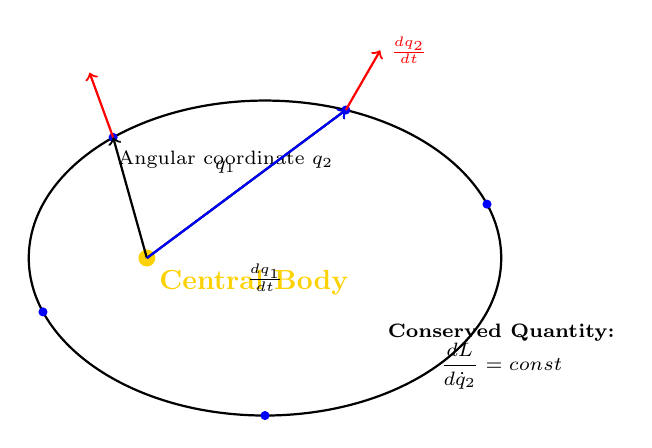
\begin{tikzpicture}[scale=2.5]

  % Draw the orbit path (elliptical trajectory)
  \draw[thick] (0,0) ellipse (1.2 and 0.8);

  % Central body (e.g., Sun)
  \filldraw[yellow!70!orange] (-0.6,0) circle (0.04) node[below right=1pt] {\textbf{Central Body}};

  % Positions along the orbit
  \foreach \angle in {20, 70, 130, 200, 270} {
    \coordinate (P\angle) at ({1.2*cos(\angle)}, {0.8*sin(\angle)});
    \filldraw[blue] (P\angle) circle (0.02);
  }

  % Labeling generalized coordinates
  \draw[->, thick] (-0.6,0) -- (P70) node[midway, above left] {\scriptsize $q_1$};
  \draw[->, thick] (-0.6,0) -- (P130);
  \node at (-0.2,0.5) {\scriptsize Angular coordinate $q_2$};

  % Tangent arrows
  \draw[->, red, thick] (P70) -- ++(60:0.35) node[right] {\scriptsize $\frac{dq_2}{dt}$};
  \draw[->, red, thick] (P130) -- ++(110:0.35);

  % Radial arrows
  \draw[->, blue, thick] (-0.6,0) -- (P70);
  \node at (0.0,-0.1) {\scriptsize $\frac{dq_1}{dt}$};

  % Angular momentum note
  \node[align=center] at (1.2,-0.5) {
    \scriptsize \textbf{Conserved Quantity:} \\
    \scriptsize $\displaystyle \frac{dL}{d\dot{q}_2} = \text{const}$
  };

\end{tikzpicture}
\caption{Lagrange's generalized coordinate system: $q_1$ (radial) and $q_2$ (angular) describe motion. Since the Lagrangian does not depend explicitly on $q_2$, the quantity $\frac{dL}{d\dot{q}_2}$ is conserved—capturing the spirit of Kepler’s Second Law.}
\end{figure}




